%\documentclass[../main.tex]{subfiles}
%\begin{document}
Process mining is a relatively new discipline that has emerged from the need to bridge the gap of data mining and business process management. The objective of process mining is to support the analysis of business process, provide valuable insights on processes and further improve the business execution. According to \cite{van2011process}, techniques of process mining are divided into three categories: process discovery, conformance checking and process enhancement. Process discovery techniques focus on deriving process models from event logs of the information system, allowing the vision into the real business process. Conformance checking analyzes the deviations between an referenced process model and observed behaviors driven from its execution. Enhancement adapts and improves existing process models by extending the model with additional data perspectives or repairing the existing model to accurately reflect observed behaviors. 

Due to the increasing availability of detailed event logs of information systems, process mining techniques have recently enabled wider applications of process mining in organizations around the world\cite{van2011process}.  After applying process discovery in organizations, a process model is fixed in information system to guide the execution of business. However,in real life, business processes often encounter exceptional situations where it is necessary to execute process differing from the predefined model. To reflect the reality, the organizations need to adapt the existing process model. Basically, one can apply process discovery techniques again to obtain a new model from event log. However, due to the facts, (1) the cost of rediscovery, and (2)  the discovered model tend to have less similarity with the original model\cite{fahland2012repairing}. As shown in \cite{fahland2012repairing}, there is a need to change an existing model similar to the original model while replaying the current process execution. Here comes the model repair. 

Model repair belongs to process enhancement and stands between process discovery and conformance checking. It analyzes the workflow deviations between event log  and process model, and fix the deviations mainly by adding sub processes on the model. As known, business in organizations is goal-oriented and aims to have high performance according to a set of Key Performance Indicators(KPIs), for example, average conversion time for the sales, payment error rate for the finance. However, there are few researches on applying the process mining with consideration of performance\cite{ghasemi2016process}.  \cite{ghasemi2016process} points out the rare contributions like \cite{dees2017enhancing} to combine performance into process mining. Deviations are firstly analyzed to determine if they have a positive impact on the process performance. Model repair techniques in \cite{fahland2015model} are applied into traces with positive deviations.

However, the current repair methods have some limits. Model repair fixes the model by adding subprocesses, silent transitions or loops, it guarantees the model fitness but overgeneralizes the model, such that it allows more behaviors than expected. On the other hand, it increases the model complexity.  Even the performance is considered in \cite{dees2017enhancing}, but only deviations in positive is used to add subprocesses, the negative information is ignored, which disables the possibility to block negative behaviors from model.  A motivation example is listed to describe those limits.
%% Motivation 
\begin{wrapfigure}{r}{0.3\textwidth}
	\centering
	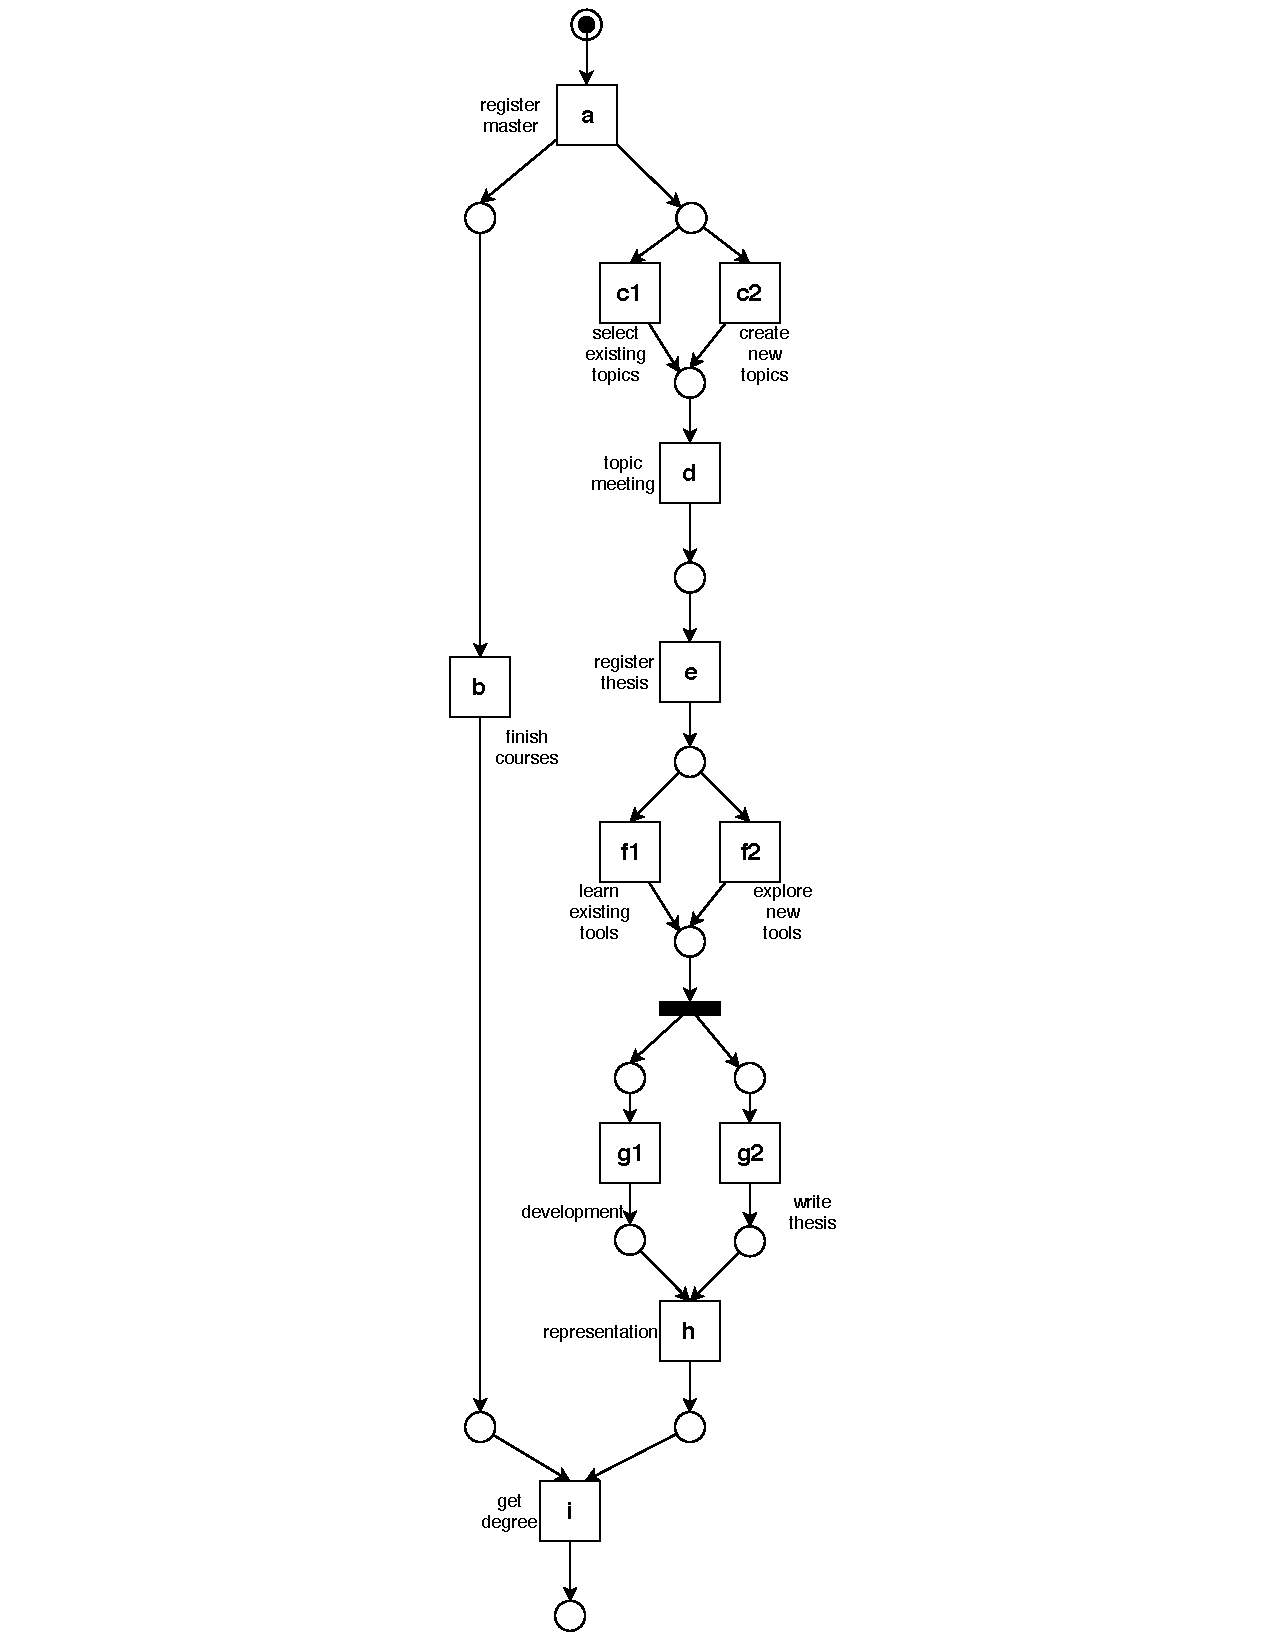
\includegraphics[clip, trim=7cm 0cm 7cm 0cm, width=0.45\textwidth, height=0.7\textheight]{figures/introduction/Master-original-model.pdf}
	\caption{original registration process}
	\label{fig:model_a}
\end{wrapfigure}
\section{Motivation Example}
% In this section, we use thesis registration example to display the shortcomings of existing techniques and then introduces our methods, but we need to answer them later..
This section describes some situations where current repair techniques can't handle properly. For the sake of understanding, some examples are extracted from the registration procedure of thesis project at one German university to illustrate those situations.

The main activities for the registration process include topic selection, make proposal, meeting with supervisor to discuss the topic, and finish course requirements. After finishing all of those activities, the formal registration is enabled and the procedure comes to end. Figure \ref{fig:model_a}  shows the original process in Petri net. The activities are modeled by the corresponding \textbf{\emph{transitions}} which is represented by a square. Transitions are connected through a circle called \textbf{\emph{place}}. Transitions and places build the static structure of Petri net. \textbf{\emph{Tokens}} in the black dot are put in the initial places and represent the dynamic state of the model. 

The model in Figure \ref{fig:model_a} is in an initial state where only one token is at the start place to enable the first transition begin thesis. After firing \emph{begin thesis}, the token at the initial place is consumed while two new token are generated in the output places. In this way, activity \emph{finish course requirements}  can be executed in concurrency with the other activities except for the \emph{register thesis}. When multiple activities have the same input place, all of them are enabled but only one of them can be fired and executed, namely, they are exclusive to each other. As shown in the figure,  \emph{select existing topics}  and \emph{create new topics} are exclusive, and only one of them can be triggered. When a transition have multiple input places, it can be triggered with condition that all input places hold at least a token. \emph{Register thesis} is enabled only after \emph{finish course requirements} and getting the \emph{approve} done. 


% here we are going to talk about the situations where the current repair method can not handle well.
In the following part, those situations are introduced to demonstrate the shortcomings of current techniques. 
\subsection{Situation 1: \small{repair model with unfit traces}} % add preparation to this model
Following the given model, in order to address the work between \emph{make proposal} and before the activity \emph{topic meeting}, two exclusive activities \emph{prepara carefully} and \emph{prepara casually} are executed in the real life and constitutes the actual event log $L_1$ listed below. With those two activities, it makes the whole procedure more efficient and clear and the traces with them are considered positive. For convenience, alphabet characters are used to represent the corresponding activities and annotated in the model. \textbf{e1, e2} represent the activities \emph{prepare carefully} and \emph{prepare casually}.\\
\emph{Event Log $L_1$ -- }
		\begin{align*}
		Positive:\{ & { <a,b, c1,d,\textbf{e1},f,g1,g2,h,i>}^{50}, \\   &{<a,b, c2,d,\textbf{e2},f,g2,g1,h,i>}^{50} \}
		% Negative: \{ & {<a,c1,d,\quad f,g1,h>}^{50} \}
		\end{align*}
\begin{figure}[htp]
	\centering
	\begin{subfigure}[b]{0.5\textwidth}
		\centering
		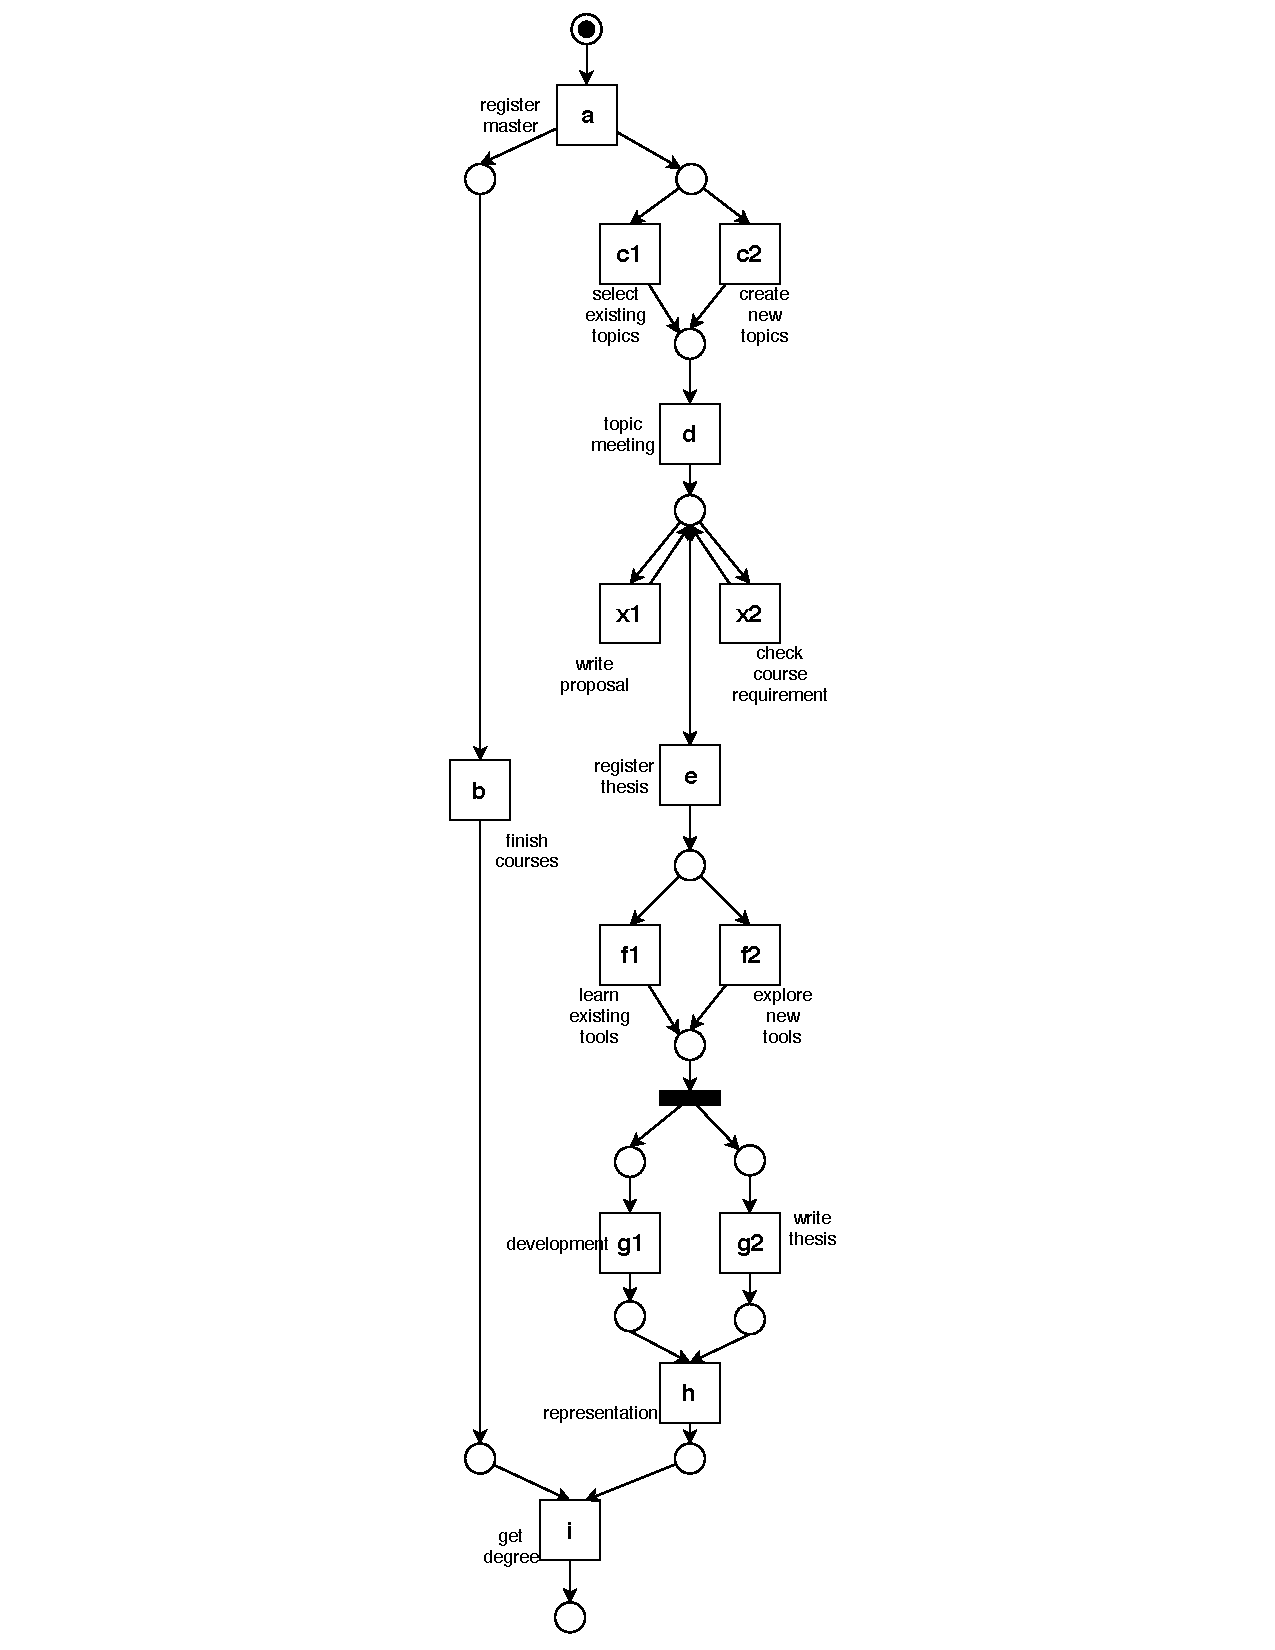
\includegraphics[clip, trim=7cm 0cm 7cm 0cm, width=0.5\linewidth, height=0.7\textheight]{figures/introduction/Master-add-events-loop.pdf}
		\caption{repaired model with additional activities }
		\label{fig:model_b1}
	\end{subfigure}%
	\begin{subfigure}[b]{0.5\textwidth}
		\centering
		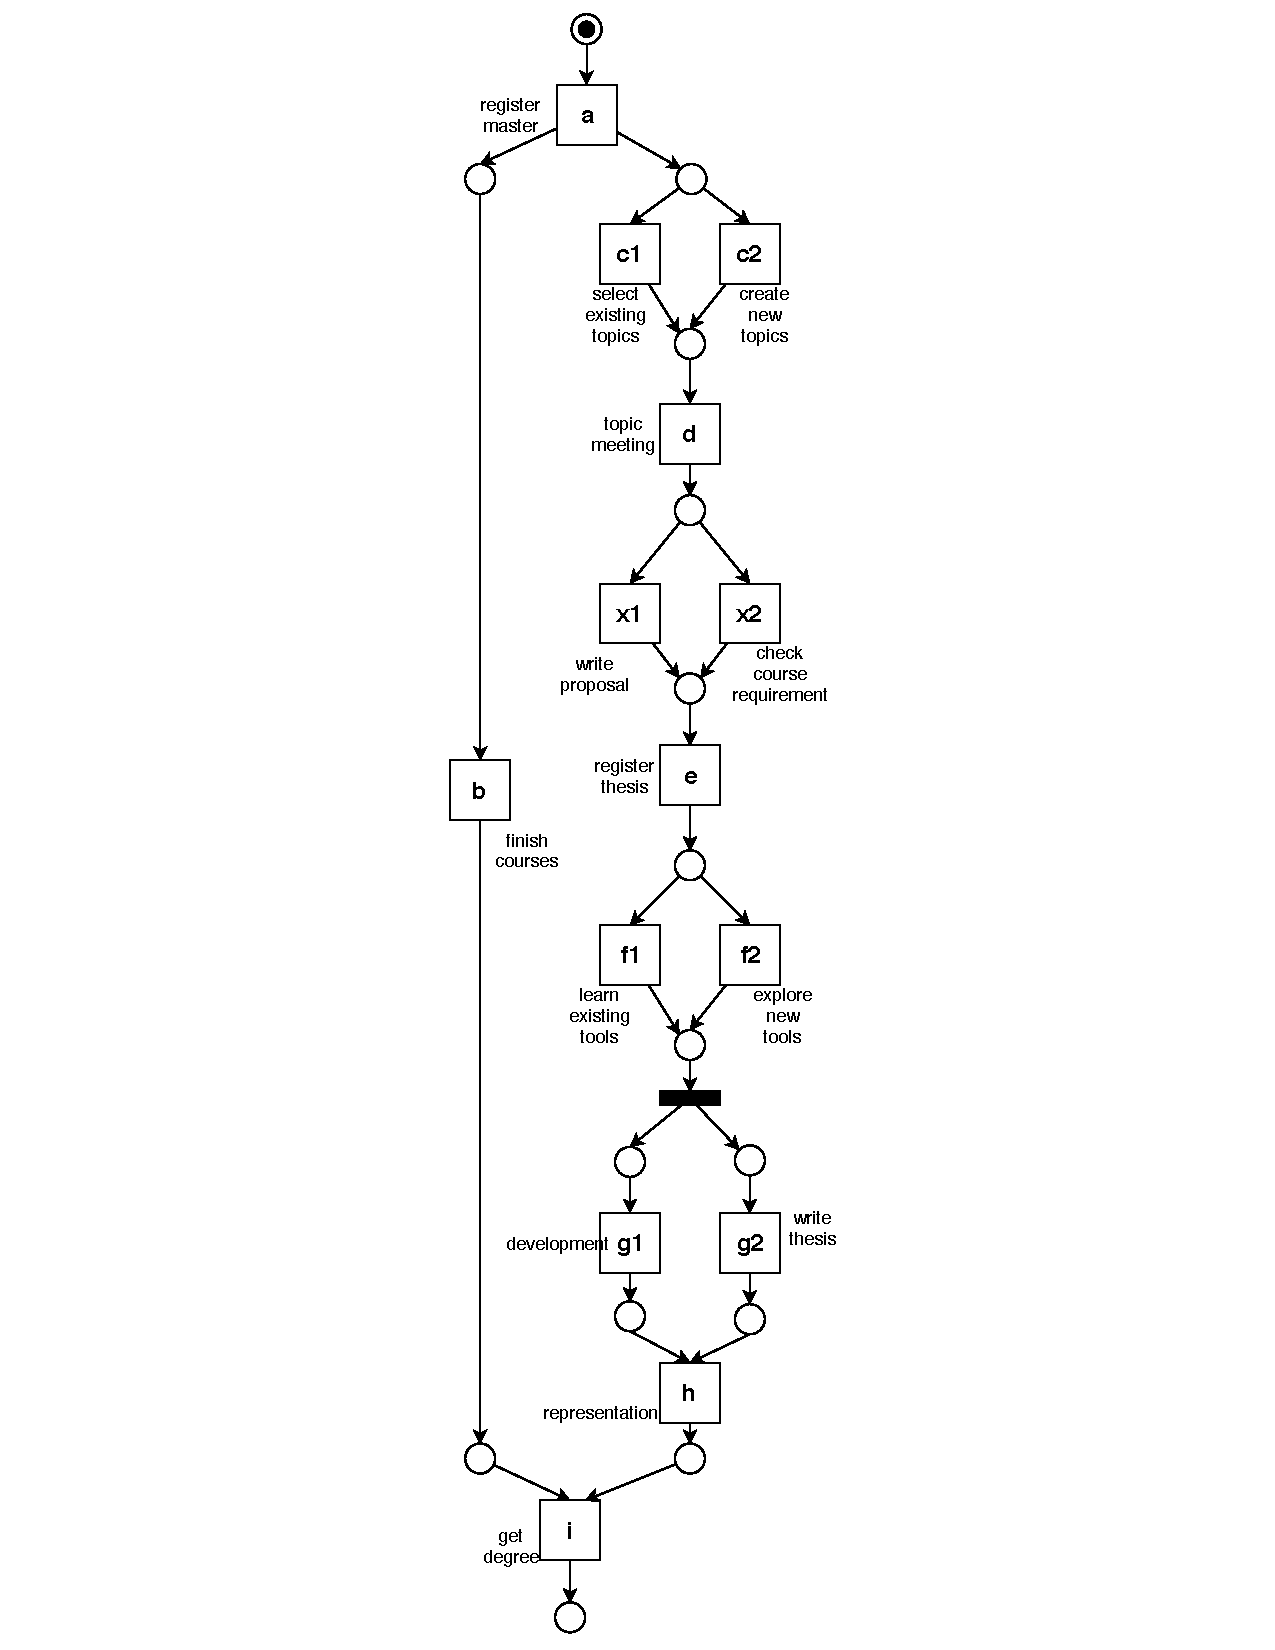
\includegraphics[clip, trim=7cm 0cm 7cm 0cm, width=0.5\linewidth, height=0.7\textheight]{figures/introduction/Master-add-events.pdf}
		\caption{expected model with additional activities}
		\label{fig:model_b2}
	\end{subfigure}
	\caption{example for situation 1}
	\label{fig:model_change_1}
\end{figure}
Because the repair techniques in \cite{fahland2015model} don't distinguish the performance of event log, to make the model enforcing the positive performance, only positive instances are employed to repair the model. Firstly, the deviations of the existing model in Figure \ref{fig:model_a} and the event log $L_1$ is computed. After computation of deviations, each deviation has the same start and end place and two deviations appear at the same position of model. When repairing this model, each subprocess has one place as its start and end place, which forms a loop in the model. If there is only one such subprocess, the subprocess will be added in an sequence in the model. This leads to a higher precision. Yet the algorithm does not discover orderings between different subprocesses at overlapping locations. So subprocesses are kept in loop form. 

The repaired model is shown in Figure \ref{fig:model_b1}, where the two additional activities are added in the form of loop.  Compared to the model in Figure \ref{fig:model_b2} where the two extra activities are shown in sequence with others, the repaired model in Figure \ref{fig:model_b1} has less precision.
% The reason why it repairs like this way 

% we need to talk about the problem in Dee's method. 
The repair algorithm in \cite{dees2017enhancing} builds upon \cite{fahland2015model} and considers the performance of event log. However, the repaired model is the same as the one in Figure \ref{fig:model_b1}. The reasons are: (1) there is no deviation from negative factors. (2) positive deviations are used in the same way like \cite{fahland2015model}. As a conclusion, the repair techniques in \cite{dees2017enhancing} can't deal with situation 1 properly, either. 

\subsection{Situation 2: \small{repair model with fit traces}}
% we should delete the prepare carefully and casually from the model. Only consider to add the data about the order change..what we expect is not 
This situation describes the existing problem in the current methods that fit traces with negative performance outcomes can not be used to repair model. Given an actual event log $L_2$, when activity \emph{finish course requirements} is fired after \emph{begin thesis} and before the topic selection part, it reduces the pressure of master thesis and has a positive outcome. Else, the negative outcomes are given. 
\emph{Event Log $L_2$ -- }
\begin{align*}
Positive:\{ & { <a,\textbf{b},c1,d,f,g2,g1,h,i>}^{50}, \\   &{<a,\textbf{b},c2,d,f,g1,g2,h>}^{50} \}  \\
Negative: \{ & {<a,c1,d,f,g2,g1,\textbf{b},h,i>}^{50}, \\
& {<a,c1,\textbf{b},d,f,g1,g2,h,i>}^{50},  \}
\end{align*}
Compared to the model, the event log $L_2$ contains no deviation. When we apply the techniques in \cite{fahland2015model} and \cite{dees2017enhancing} to repair the model, the model keeps untouched due to no deviation. Apparently, those two methods can't incorporate the negative information in fit traces. When we expect a model which enforce the positive instances and avoid the negative instance as the model in Figure \ref{fig:model_c}, the current methods fail our need. 
\begin{figure}[htp]
	\centering
	\begin{subfigure}[b]{0.5\textwidth}
		\centering
		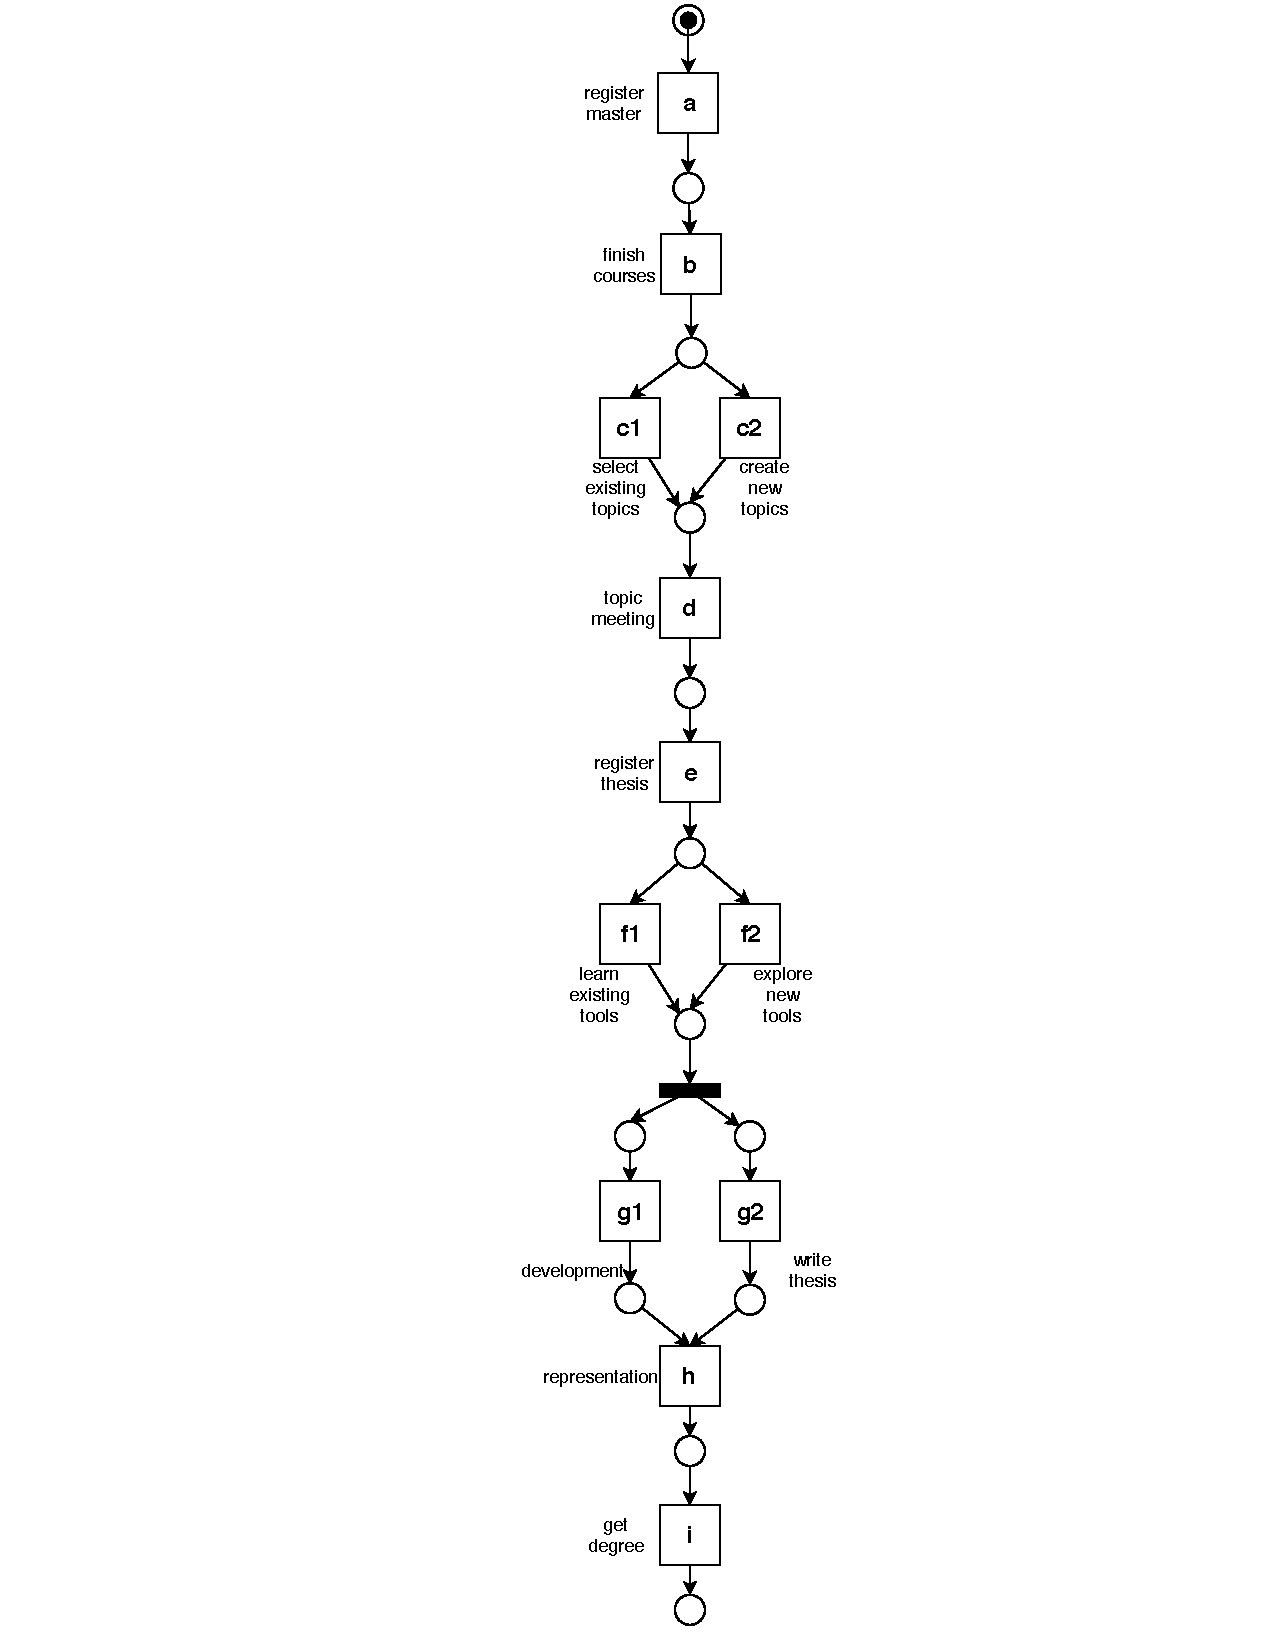
\includegraphics[clip, trim=8cm 0cm 8cm 0cm, width=0.5\linewidth, height=0.7\textheight]{figures/introduction/Master-change-order.pdf}
		\caption{expected model with order change}
		\label{fig:model_c}
	\end{subfigure}%
	\begin{subfigure}[b]{0.5\textwidth}
		\centering
		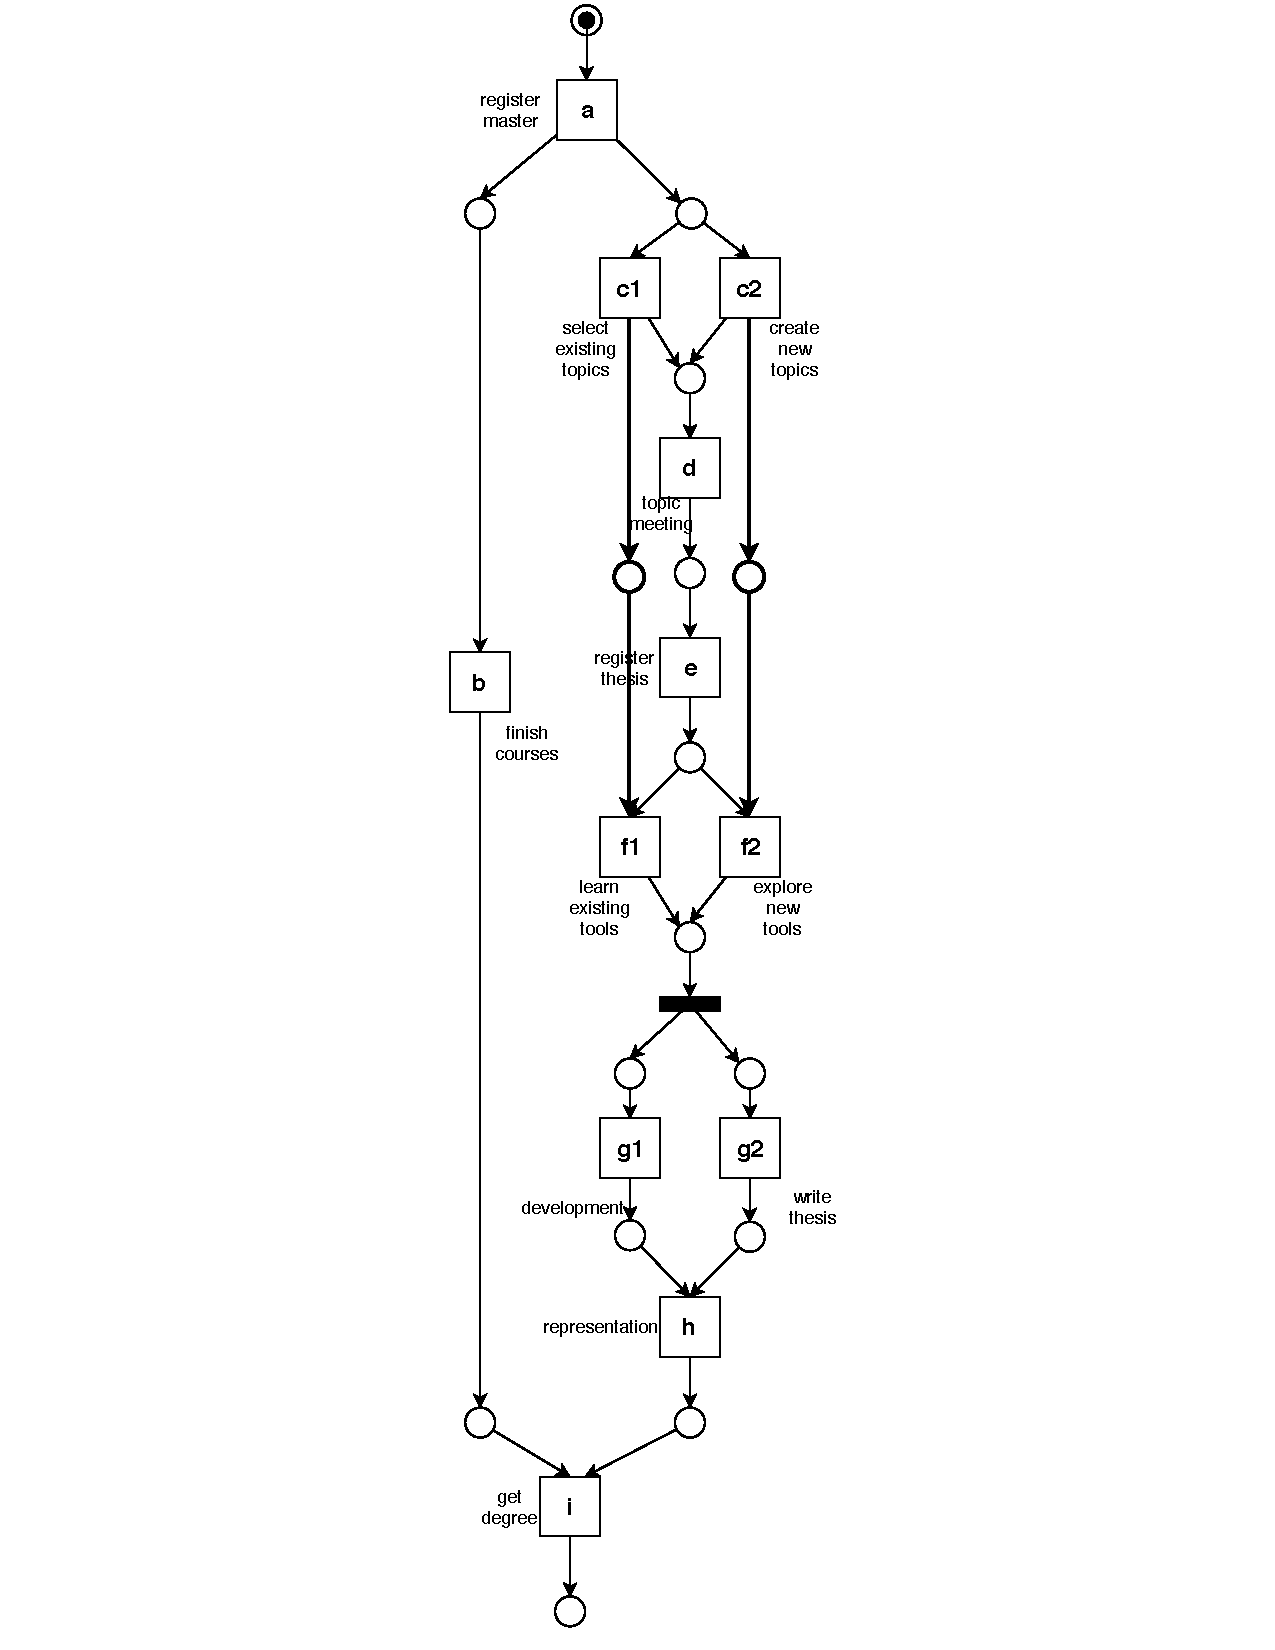
\includegraphics[clip, trim=7cm 0cm 7cm 0cm, width=0.5\linewidth, height=0.7\textheight]{figures/introduction/Master-with-lt.pdf}
		\caption{model with long-term dependency}
		\label{fig:model_d}
	\end{subfigure}
	\caption{example for situation 2 and 3}
	\label{fig:model_changes_2_3}
\end{figure}
\subsection{Situation 3: \small{detect long-term dependency}}
This part introduces a problem which causes a lower precision in process model. It is the inability in current methods to detect the long-term dependency in the Petri net. The long-term dependency describes the phenomenon that one execution choice decides the execution of activities that do not follow directly. Due to the long distance of this dependency, current methods can not detect it and improve the precision by adding long-term dependency on model. 
An event log $L_3$ is given in the following. By using time consumption as one KPI, if the total sum goes over one threshold, we mark this trace as negative, else as positive. Since \emph{create new topics} usually demands new knowledge rather than checking the existing tools. So if student chooses to learn existing model, it's possibly not useful and wastes time. In the other case, if we select existing topics with existing background, it saves time when we directly learn the existing tools. According to this performance standard, we classified those event traces.
\emph{Event Log $L_3$ -- }
\begin{align*}
Positive:\{ & { <a,b,\textbf{c1},d,e,\textbf{f1},g1,g2, h,i>}^{50}, \\   &{<a,b,\textbf{c2},d,e,\textbf{f2},g2,g1, h,i>}^{50} \}  \\
Negative: \{ & {<a,b,\textbf{c1},d,e,\textbf{f2},g2,g1,h,i>}^{50}, \\
& {<a,b,\textbf{c2},d,e,\textbf{f1},g1,g2,h,i>}^{50}  \}
\end{align*}
%here we list one example to explain the long-term dependency, but we need to make them clear, might without the loop item..It means that we need to change the whole model..
There is no deviations of the model and event log $L_3$ according to the  algorithms in \cite{fahland2015model} and \cite{dees2017enhancing}. Therefore, the original model stays the same and allows the execution of negative instances. After checking the model and log, two long-term dependency have significant evidence. Transition \textbf{\emph{c1}} decides \textbf{\emph{f1}} while \textbf{\emph{c2}} decides \textbf{\emph{f2}}.  After addressing long-term dependency like the model in Figure \ref{fig:model_d} by connecting transitions to extra places, 
negative instances are blocked and the model has a higher precision.

Clearly, the use of negative information can bring significant benefits, e.g, enable a controlled generalization of a process model: the patterns to generalize should never include negative instances. The demand to improve current repair model techniques with incorporating negative instances appears. In the next section, the demand is analyzed and defined in a formal way.

\section{Research Problem And Questions}
We analyze the current model repair methods, and give the formal definitions.
\begin{definition}
Given an input of one existing process model M, an event log L with performance outcomes, how  to improve current process enhancement techniques by incorporating negative information, and generate a process model to enforce the positive instances while blocking the negative instance, with condition that the generated model should be as similar to the original model as possible Therefore, the repaired model provides a better way to understand and execute the real business process compared to the original model.
\end{definition}
\begin{figure}
	\centering
	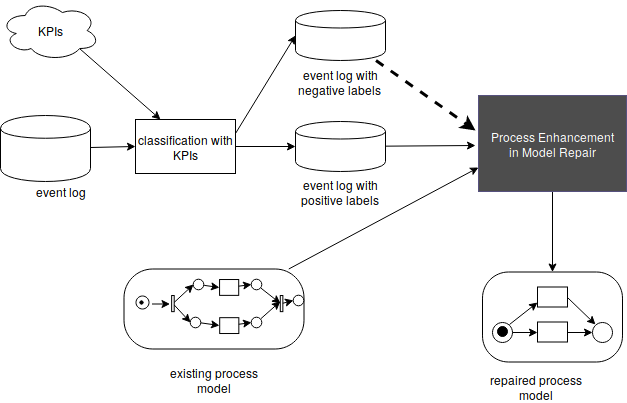
\includegraphics[width=\textwidth]{figures/introduction/FD_approach_blackbox.png}
	\caption{The problem description}
	\label{fig:method_architecture}
\end{figure}
An event log and an existing model are given as the input. According to some predefined KPIs, each trace in event log is classified into positive or negative. After applying repair techniques in the black box, the model should be improved to enforce the positive instances while disallowing negative instance.  

This paper tries to provide a solution for the black box. Our idea is to analyze the positive and negative impact on process performance of each trace. It balances the existing model, positive traces and negative traces on directly-follows relation, in order to incorporate all the factors on model generation. Later, the directly-follows relation is used to create process model by Inductive Miner. What's more, the impact of the existing model, positive and negative instances are parameterized by weights, to allow more flexibility of the generated model.

\section{Outline}
The reminder is organized in the following order. Section 2 recalls the basic notions on process mining and list the preliminary to solve the problem. The next section lists our methods are introduced and formal definitions are given. In Implementation Section, the details of algorithms are given. Later, we evaluate our methods with simulated data and real data respectively and list the results. Subsequently, the discussion on this paper is presented. At last section, a conclusion is drawn on the paper. 


%\end{document}